\renewcommand{\chaptername}{Capitulo}
\chapter{Marco Te\'orico} 
\section{Metadatos}

Actualmente, en la web existe gran cantidad de informaci\'on sobre cualquier tema, tanta que se requiere del desarrollo de servicios que consideren su pertinencia, veracidad y  calidad para satisfacer necesidades de informaci\'on espec\'ificas de los usuarios, as\'i como, considerar aspectos de accesibilidad y disponibilidad, dado que los usuarios acceden desde cualquier lugar y mediante una gama amplia de dispositivos.

El etiquetado y descripci\'on de los contenidos son cruciales en el desarrollo de este tipo de servicios, el primero permite categorizar o clasificar la informaci\'on, el segundo se refiere al uso de las descripciones o elementos descriptores, denominados \emph{metadatos}, para que las p\'aginas web se localicen y procesen adecuadamente por un agente tal como una computadora, una aplicaci\'on m\'ovil u otro tipo de programa. Seg\'un \cite{W3C}, una prioridad particular del \emph{World Wide Web Consortium}, (Consorcio W3C), es usar la web para documentar el significado de los metadatos. El inter\'es en los metadatos 
y en modelos sem\'anticos de representaci\'on de conocimiento u ontolog\'ias, ha impulsado el desarrollo del modelo de datos conocido como Marco de Descripci\'on de Recursos, en ingl\'es \emph{Resource Description Framework} o RDF. 

\section{El modelo de datos RDF en el contexto de las tecnolog\'ias de la web sem\'antica}

La \textit{World Wide Web} o simplemente la \textit{web}, es una plataforma tecnol\'ogica que constituye la mayor base de datos existente, se conforma por todo tipo de recursos, donde una persona o tambi\'en llamada usuario, publica, explora, consulta o guardar informaci\'on. Inicialmente, la web s\'olo almacenaba recursos entendibles para los seres humanos sin considerar que, con el paso del tiempo, es de suma importancia su gesti\'on autom\'atica por computadoras. 

La web sem\'antica, extensi\'on de la web tradicional, promueve el modelado, etiquetado y representaci\'on de la informaci\'on de manera que tanto los humanos como las computadoras sean capaces de \textit{comprender} el contenido de una p\'agina o recurso.

\begin{figure}[!ht]
    \centering
    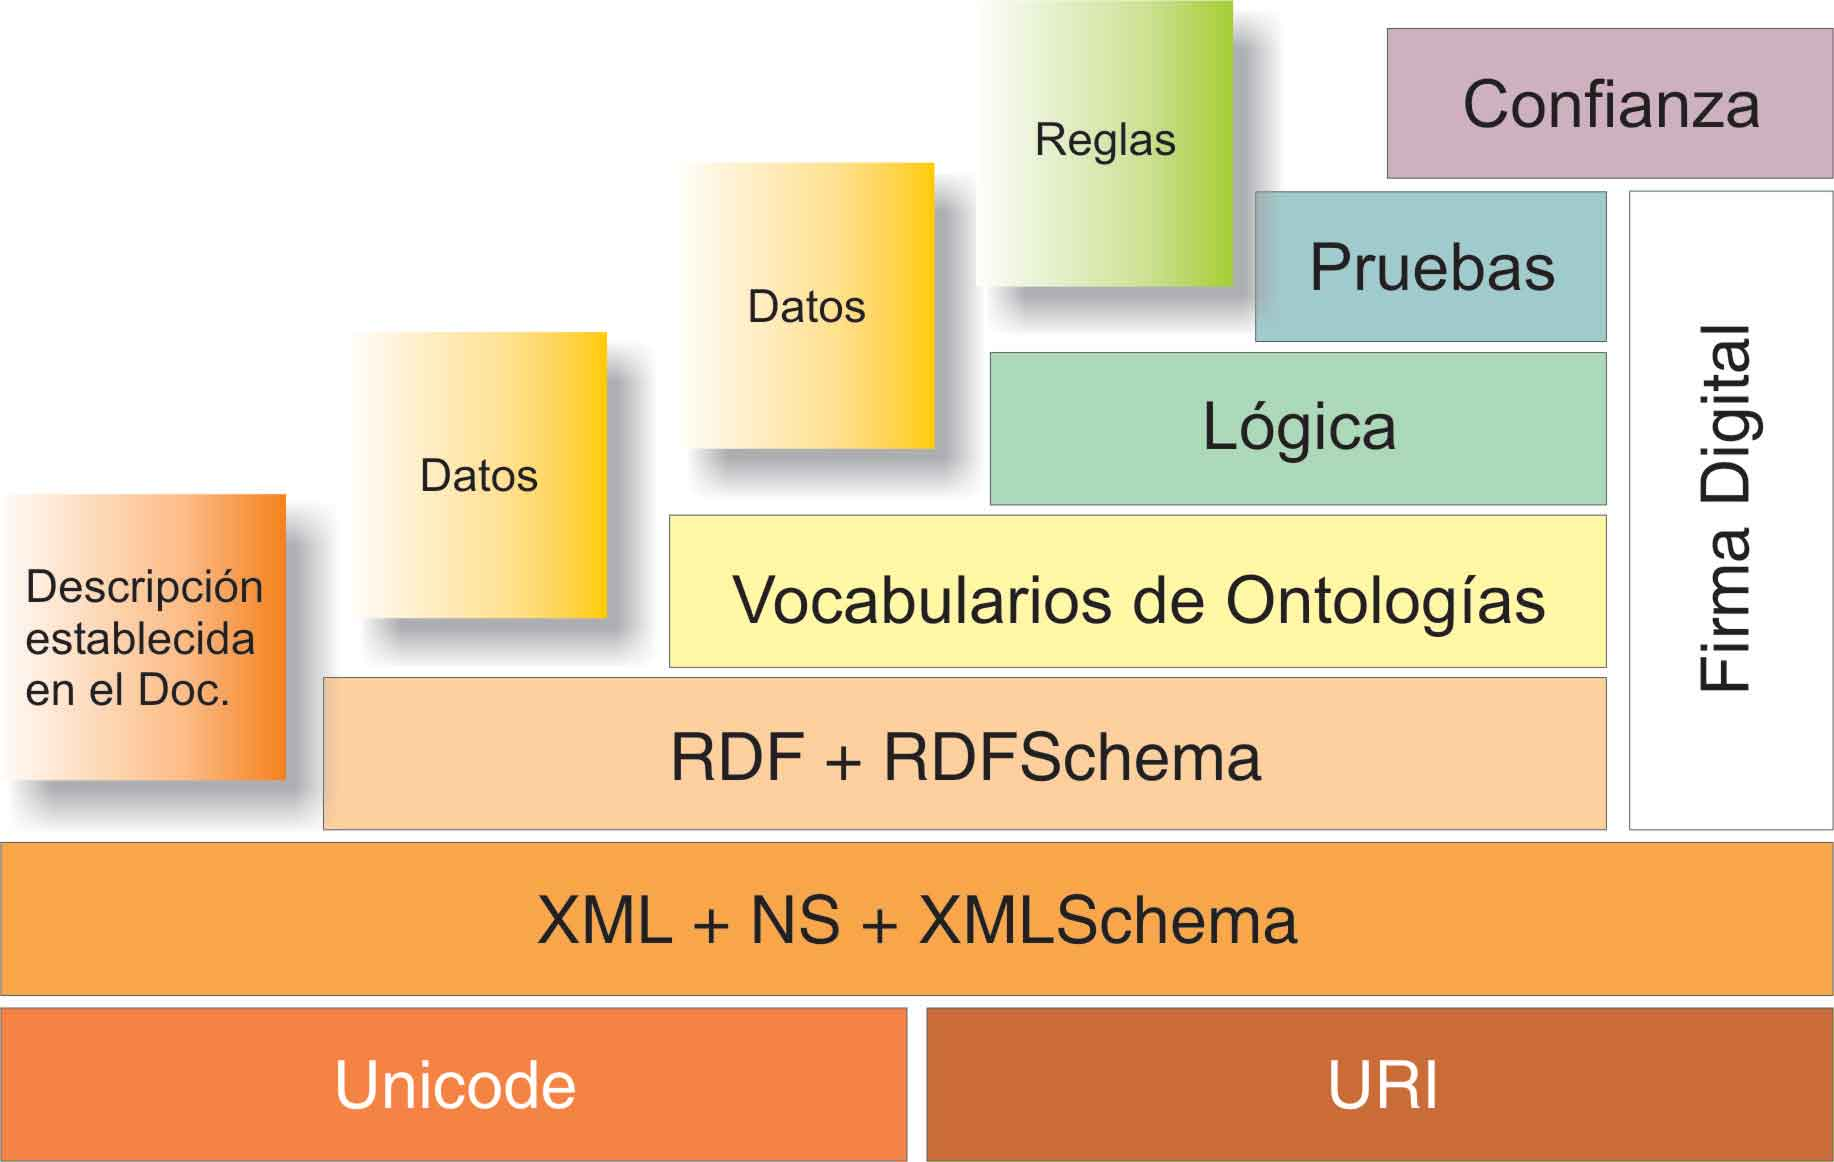
\includegraphics[width=10cm]{figures/ModeloCapasWebSemantica.jpg} %NOMBRE DE LA FIGURA y TAMAÑO
    \caption{Modelo de capas de Berners-Lee para la web sem\'antica\cite{WebSemantica_SciELO}} %PIE DE LA IMAGEN
    \label{Modelo_Web_Semantica}
\end{figure}

La web sem\'antica, como menciona \cite{IntroBD_RDF}, propone una alternativa para agregar significado a los contenidos almacenados en la web, lo cual propicia una interacci\'on m\'as fluida entre aplicaciones, servicios, computadoras y el ser humano en comparaci\'on con la web tradicional. 

Las tecnolog\'ias de la web sem\'antica se rigen bajo ciertas normas y lenguajes est\'andar organizados en capas o niveles, como muestra la figura \ref{Modelo_Web_Semantica}, los cuales se describen a continuaci\'on: \cite{IntroBD_RDF}

\begin{itemize}
    \item \textit{Unicode} \cite{W3C}. Est\'andar para documentos de texto que permite codificar la mayor\'ia de los sistemas de escritura del mundo.
    
    \item \textit{URI\footnote{\textit{Uniform resource identifier} (Identificador uniforme de recursos)}} \cite{W3C}. Est\'andar para crear identificadores de recursos Web a trav\'es de cadenas compactas de caracteres que permiten su identificaci\'on un\'ivoca y localizaci\'on autom\'atica. Un URL\footnote{\textit{Uniform Resource locator} (identificador de recursos uniforme)} es un tipo de URI, por ejemplo, \texttt{http://informatica.uppuebla.edu.mx/~mmedina/} identifica espec\'ificamente un recurso, es este caso, la p\'agina inicial de una persona. 
    
    \item \textit{XML\footnote{\textit{eXtensible Markup language} (Lenguaje de Marcado Extensible o Lenguaje de Marcas Extensible)}} \cite{W3C}. Es un lenguaje de marcado similar a HTML, es una especificaci\'on del W3C de prop\'osito general, por lo que cada usuario define sus propias etiquetas. 
    
    \item \textit{XML Namespaces} (Espacios de nombre de XML) \cite{W3C}. Es una recomendaci\'on W3C, la cual a trav\'es de etiquetas se clasifican los t\'erminos de un documento XML, de manera que cada t\'ermino est\'a identificado por una URI que lo hace \'unico y universal. Los espacios de nombres se emplean para atender el problema de ambig\¨uedad en los documentos XML de la web.
    
    \item \textit{RDF}\footnote{\textit{Resource Description Framework} (Marco de descripci\'on de recursos)} \cite{W3C_SemanticWeb}. Modelo est\'andar para el intercambio de datos en la web, con caracter\'isticas que facilitan la fusi\'on de datos inclusive si los esquemas subyacentes son diferentes. RDF ampl\'ia la estructura de enlaces web (\emph{links}), para nombrar a dos recursos, denominados sujeto y objeto, as\'i como la relaci\'on entre el sujeto y el objeto. Estos enunciados se conocen como \textit{ternas}). En el modelo de datos RDF se representan datos estructurados y semiestructurados o combinaciones de ambos, los cuales se comparten y utilizan por diferentes aplicaciones.
    
    \item \textit{RDF Schema} \cite{W3C_RDFSchema}. Proporciona un vocabulario del modelado de datos para RDF, lo complementa con diferentes documentos anexos que describen los conceptos b\'asicos y la sintaxis abstracta de RDF. RDF Schema es una extensi\'on sem\'antica de RDF que proporciona mecanismos para describir grupos de recursos relacionados y sus relaciones. Schema RDF est\'a escrito en RDF, los recursos se utilizan para determinar las caracter\'isticas de otros recursos como dominio y rangos de propiedades.
    
    %%DANIEL, FALTA COMPLETAR ESTAS DEFINICIONES
    
    %\item \textit{Ontolog\'ia}. Seg\'un \cite{Ontologias}, una ontolog\'ia es un marco com\'un o una estructura conceptual sistematizada y de consenso no s\'olo para almacenar la informaci\'on, sino tambi\'en para poder buscarla y recuperarla. Una ontolog\'ia define los t\'erminos y las relaciones b\'asicas para la compresi\'on de un \'area del conocimiento, as\'i como las reglas para poder combinar los t\'erminos para definir las extensiones de este tipo de  vocabulario controlado.
    
    \item \textit{Vocabularios de ontolog\'ias}. El Lenguaje de Ontolog\'ias Web (OWL) est\'a diseñado para ser usado en aplicaciones que necesitan procesar el contenido de la informaci\'on en lugar de \'unicamente representar informaci\'on para los humanos. OWL representa a interpretar de manera m\'as adecuada los contenidos Web a diferencia de XML, RDF, y RDF Schema, ya que  proporciona vocabulario adicional junto con una sem\'antica formal. OWL tiene tres sublenguajes, con un nivel de expresividad creciente: OWL Lite, OWL DL, y OWL Full. \cite{LaWebSemantica}
    
    \item \textit{Capa l\'ogica}. Permite determinar si la estructura de los razonamientos es v\'alida a trav\'es del estudio de las reglas formales. Permite realizar consultas e inferir conocimiento, por medio de la interacci\'on entre las ontolog\'ias y los agentes software (programas o aplicaciones). \cite{LaWebSemantica}
    
    \item \textit{Capa de pruebas}. A trav\'es de demostraciones matem\'aticas se comprueba que el procesamiento del agente de software alcanz\'o la m\'axima confiabilidad en sus razonamientos. \cite{LaWebSemantica}
    
    \item \textit{Capa de confianza}. Es una capa que establece las pol\'iticas de seguridad que permitan asignar niveles de fiabilidad a determinados recursos, de forma comprobable posteriormente por los agentes, para lo que se usar\'an firmas digitales y redes de confianza. \cite{LaWebSemantica}

\end{itemize}

Los lenguajes utilizados ampliamente para representar los datos en la web sem\'antica son XML, RDF y OWL.\newline

\section{SPARQL}

RDF es un modelo de datos que se asocia con diferentes representaciones, una de ellas es como un modelo de grafos dirigidos etiquetados que representan informaci\'on en la web. Se emplea para representar de informaci\'on personal, redes sociales, metadatos sobre objetos digitales o como medio para la integraci\'on de fuentes de informaci\'on heterog\'eneas.

Los datos en RDF se recuperan utilizando SPARQL, \textit{SPARQL protocol and RDF query language}, protocolo y lenguaje de consulta para RDF, est\'a orientado a datos, sirve para extraer la informaci\'on contenida en el modelo ontol\'ogico, devuelve resultados en forma de enlaces o esquemas RDF. Entre sus especificaciones, de acuerdo con \cite{Skos_Sparql}, se encuentran las siguientes:

\begin{itemize}
    \item La especificaci\'on del protocolo SPARQL para RDF \textit{SPROT} que define el protocolo remoto para enviar consultas SPARQL y recibir los resultados
    \item La especificaci\'on del formato XML de los resultados de consultas SPARQL \textit{RESULTS}, define un formato de documento XML para representar los resultados de las consultas \texttt{SELECT} y \texttt{ASK} 
\end{itemize}

La Figura \ref{ejemplo_RDF_grafico} muestra una representaci\'on gr\'afica simple de \textit{vc-db-1.rdf}, archivo que contiene RDF para varias descripciones de vCard de personas, descritas en las notas del W3C ``Representaci\'on de objetos vCard en RDF / XML''.\newline

\begin{figure}[!ht]
    \centering
    \fbox{
    \includegraphics[width=12cm]{figures/vc-db.png}} %NOMBRE DE LA FIGURA y TAMAÑO
    \caption{Ejemplo de representaci\'on gr\'afica provenientes de Representaci\'on de objetos vCard en RDF / XML} %PIE DE LA IMAGEN
    \label{ejemplo_RDF_grafico}
\end{figure}

La Figura \ref{ejemplo_RDF_ternas} muestra el esquema RDF expresado como un conjunto de ternas, (tambi\'en llamadas tripletas).\newline

\begin{figure}[!ht]
    \centering
    \fbox{
    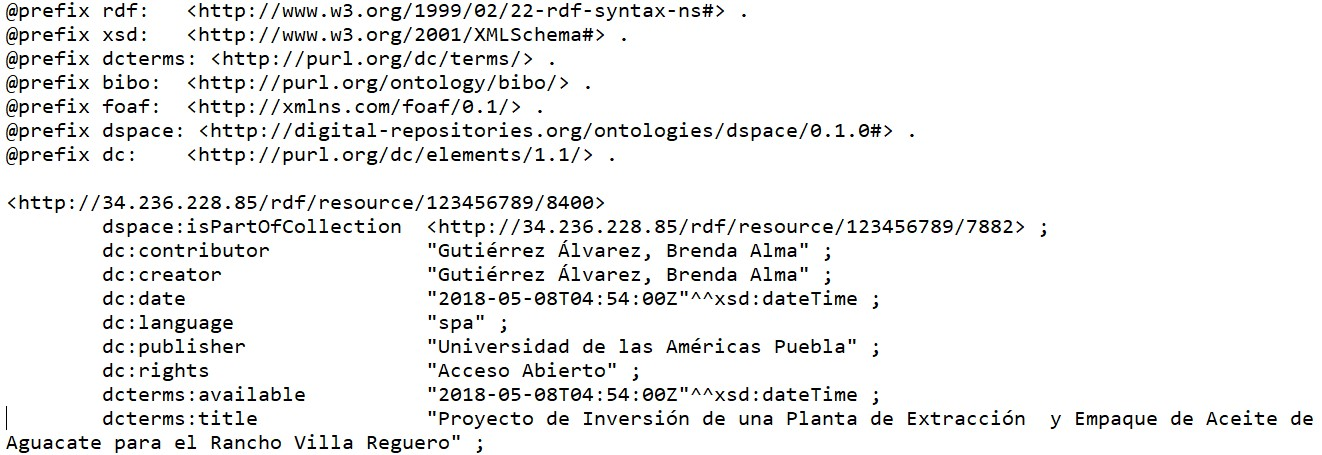
\includegraphics[width=12cm]{figures/ejemploRDF.jpg}} %NOMBRE DE LA FIGURA y TAMAÑO
    \caption{Ejemplo de conjunto de ternas en RDF} %PIE DE LA IMAGEN
    \label{ejemplo_RDF_ternas}
\end{figure}
    
\section{Servicios REST}

Los servicios REST formaron una gran opci\'on para la explotaci\'on de recursos apartir de la migraci\'on a la web 2.0, sustitutendo aquellos que hacian uso de los protocolos SOAP y WSDL, haciendo uso de una arquitectura m\'as sencilla, orientado a recursos y haciendo uso del protocolo HTTP. Los servicios REST \footnote{\textit{Representational State Transfer} (Transferencia de Estado Representacional)} cumplen con las siguientes premisas: \cite{FeaturesREST}

\begin{itemize}
    \item Se define una \textbf{interfaz} de comunicaci\'on \textbf{cliente-servidor} separando completamente las responsabilidades entre ambas partes, como se muestra en la figura \ref{arquitectura_REST_1}.
    
    \begin{figure}[!ht]
    	\centering
    	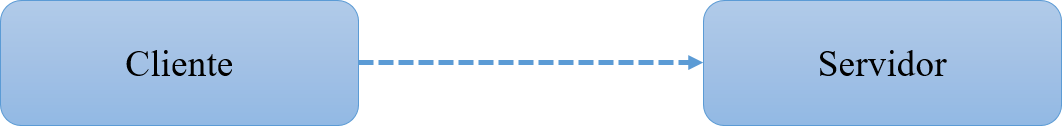
\includegraphics[width=10cm]{figures/ClienteServidorREST.png} %NOMBRE DE LA FIGURA y TAMAÑO
        \caption{Arquitectura cliente servidor de servicio REST} %PIE DE LA IMAGEN
        \label{arquitectura_REST_1}
    \end{figure}
    
    \item Servicio web \textbf{sin estado} ya que  cada petici\'on que se realiza es completamente independiente de cualquier otra, sin embargo, todas las solicitudes al mismo servicio son totalmente id\'enticas, como se muestra en la figura \ref{arquitectura_REST_2}.
    
    \begin{figure}[!ht]
    	\centering
    	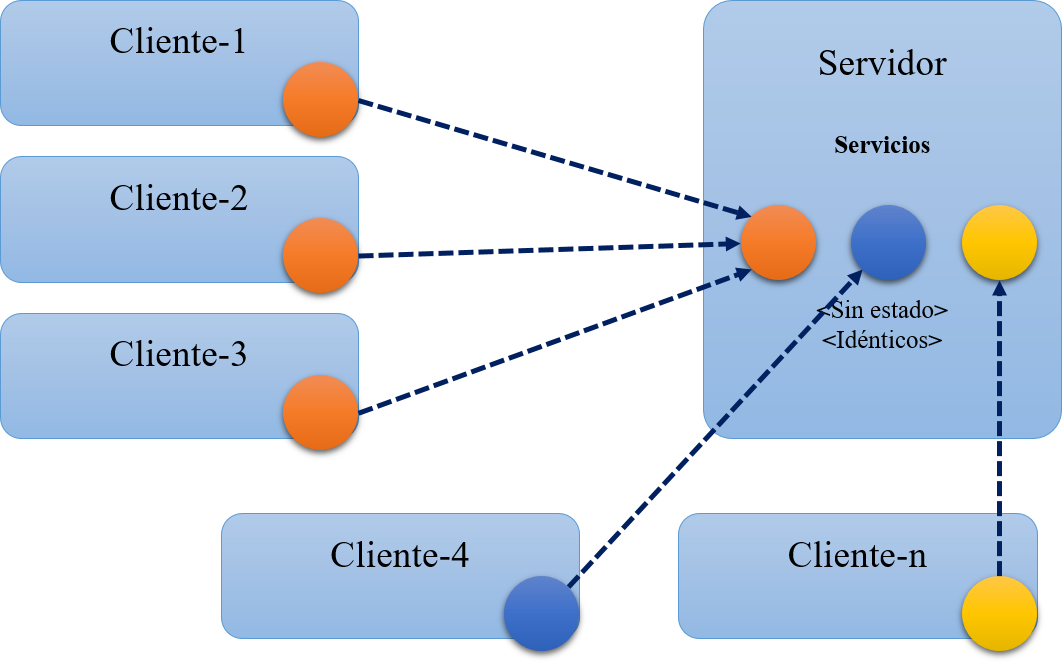
\includegraphics[width=10cm]{figures/ClienteServidorREST2.png} %NOMBRE DE LA FIGURA y TAMAÑO
        \caption{Servicios sin estado de la Arquitectura cliente servidor REST} %PIE DE LA IMAGEN
        \label{arquitectura_REST_2}
    \end{figure}
    
    \item Los servicios web REST pueden guardar en cache su contenido de tal manera que una vez realizada la primera petici\'on al servicio, el resto de peticiones puedan apoyarse en la cache si fuera necesario, como se muestra en la figura \ref{arquitectura_REST_3}.
    
    \begin{figure}[!ht]
    	\centering
    	\includegraphics[width=10cm]{figures/Cliente_servidor_REST_3.png} %NOMBRE DE LA FIGURA y TAMAÑO
        \caption{Servicios REST apoyados en cache} %PIE DE LA IMAGEN
        \label{arquitectura_REST_3}
    \end{figure}
    
    \item Todos lo servicios REST son \textbf{uniformes}, es decir, que compartir\'an una forma de invocaci\'on y m\'etodos similares utilizando los metodos GET,POST,PUT ,DELETE, como se muestra en la figura \ref{arquitectura_REST_4}.
    
    \begin{figure}[!ht]
    	\centering
    	\includegraphics[width=10cm]{figures/Cliente_servidor_REST_4.png} %NOMBRE DE LA FIGURA y TAMAÑO
        \caption{Servicios REST uniformes} %PIE DE LA IMAGEN
        \label{arquitectura_REST_4}
    \end{figure}
    
    \item Finalmente, todos los servicios REST son escalables y para el cliente REST es transparente, es decir, no ser\'a capaz de distinguir entre si la petici\'on es atendida directamente por servidor , o por el sistema de caches, a trav\'es de un servicio de balanceo de cargas, como se muestra en la figura \ref{arquitectura_REST_5}.
    
    \begin{figure}[!ht]
    	\centering
    	\includegraphics[width=10cm]{figures/Cliente_servidor_REST_5.png} %NOMBRE DE LA FIGURA y TAMAÑO
        \caption{Arquitectura de capas de los Servicios REST} %PIE DE LA IMAGEN
        \label{arquitectura_REST_5}
    \end{figure}
    
\end{itemize}

Si bien algunos repositorios institucionales (RIs) cuentan con servicios tipo REST , el grado de complejidad en las consultas que hasta el momento estan implementadas, consideran s\'olo un atributo, lo cual restringe el tipo de informaci\'on que puede recuperarse.\newline

El RN ofrece un cat\'alogo de m\'as de doscientos servicios REST \footnote{Disponible en: \textit{https://www.repositorionacionalcti.mx/docs/manualesInteroperabilidad}} que estan disponibles para aquellos usuarios que requieren informaci\'on (en formato JSON) \cite{CatalogoREST_RN} de cualquiera de los apartados mostrados en el cuadro \ref{descripcion_servicios_REST_RN}.

\begin{table}[htbp]
\caption{Cat\'alogo de servicios REST ofrecidos por el RN} %Leyenda de la tabla
\begin{tabular}{| p{7cm}| p{7cm} |} \hline
\'areas de conocimiento          & Licencia                       \\ \hline
Campos de conocimiento         & Localidad                      \\ \hline
Disciplinas de conocimiento    & Municipio                      \\ \hline
Subdisciplinas de conocimiento & Nivel de acceso                \\ \hline
Audiencia                      & Pa\'is                           \\ \hline
Estado                         & Persona                        \\ \hline
Instituci\'on                    & Formato                        \\ \hline
Idioma                         & Programa                       \\ \hline
Financiador – Programa         & Proyecto                       \\ \hline
\end{tabular}

\label{descripcion_servicios_REST_RN}
\end{table}

Para que un usuario pueda consultar alguno de los cat\'alogos de datos, es necesario identificar la b\'usqueda concreta que arroje la informaci\'on que se desea consultar. Al mismo tiempo, existen al menos sietes servicios b\'asicos de consulta y otros m\'as espec\'ificos, dependiendo del cat\'alogo. Un ejemplo de lo anterior se muestra en la figura \ref{ejemplo_consumo_REST_RN}.

\begin{figure}[!ht]
    \centering
    \fbox{
    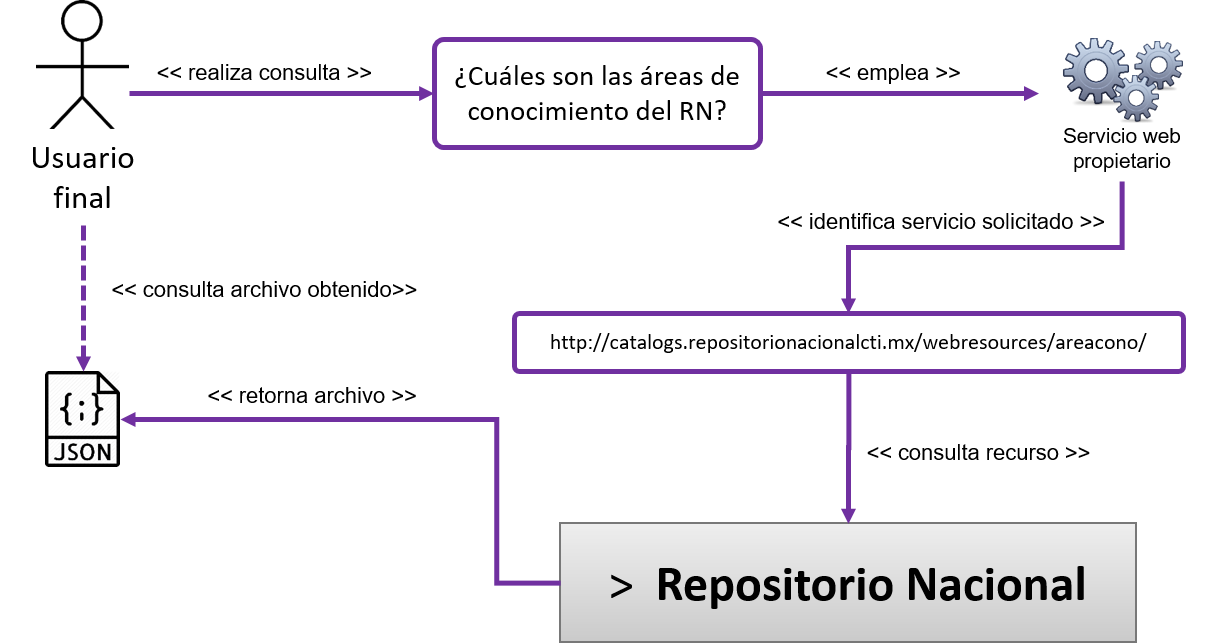
\includegraphics[width=12cm]{figures/ConsumoREST.png}} %NOMBRE DE LA FIGURA y TAMAÑO
    \caption{Ejemplo de consumo de un servicio REST del RN} %PIE DE LA IMAGEN
    \label{ejemplo_consumo_REST_RN}
\end{figure}

Finalmente, el resultado de la consulta efectuada mediante uno de los servicios REST, es un archivo en formato JSON \footnote{JSON o \textit{JavaScript Object Notation} es un  formato de texto ligero para el intercambio de datos}, como se observa en la figura \ref{JSON_ejemplo_consumo_REST_RN}.

\begin{figure}[!ht]
    \centering
    \fbox{
    \includegraphics[width=12cm]{figures/JSON_servicio_REST_RN.png}} %NOMBRE DE LA FIGURA y TAMAÑO
    \caption{Archivo tipo JSON obtenido mediante servicio REST del RN} %PIE DE LA IMAGEN
    \label{JSON_ejemplo_consumo_REST_RN}
\end{figure}

\section{COAR}

En 2016, la Confederation of Open Access Repositories - \textit{COAR} (Confederaci\'on de Repositorios de Acceso Abierto) integr\'o un equipo de trabajo llamado \textit{Next Generation Repository Working Group} (Equipo de trabajo para la siguiente generaci\'on de repositorios) cuyo porp\'osito fue el de definir las funcionalidades y tecnolog\'ias a desarrollar en los RDs en los pr\'oximos años. Derivado de estos trabajos, el informe \textit{Behaviours and Technical Recommendations of the COAR Next Generation Repositorie} \cite{NextGenerationRepositories} indic\'o que ser\'a necesario adoptar nuevas tecnolog\'ias, est\'andares y protocolos que permitan una mejor integraci\'on de los repositorios en los entornos web, de esta manera, \'estos jugar\'an un papel importante en el amplio campo de la comunicaci\'on acad\'emica.

Lo anterior dej\'o al descubierto que, hoy en d\'ia muchas de los medios de difusi\'on de la investigaci\'on y de la producci\'on acad\'emica de las IES y CI, han cubierto estas funcionalidades desde un punto de vista b\'asico, lo cual dista de ser lo ideal si lo que se pretende es darle covertura amplia y pertinente del los contenidos de los repositorios. Uno de los aspectos que no aportan a la igualdad y libre acceso a la informaci\'on, es la publicaci\'on en medios tradicionales, cuyos incentivos coorporativos ponen en desventaja a aquellos que no cuentan con acceso a sus plataformas, medios digitales o impresos.

Finalmente, el estudio plantea once caracter\'isticas importantes que los repositorios del futuro deben contemplar para establecerse como una fuente s\'olida de publicaci\'on, confiable y de AA: \cite{NextGenerationRepositories}

\begin{itemize}
\item Exponer \textit{identificadores}
\item Declaraci\'on de \textit{licencias} a nivel de recursos
\item Descubrimientos a trav\'es de la \textit{navegaci\'on}
\item Interactuar con \textit{recursos}
\item Descrubrimiento de \textit{lotes}
\item \textit{Transferencia} de recursos
\item \textit{Metadatos} de la actividad de recopilaci\'on y exposici\'on de la informaci\'on
\item \textit{Identificaci\'on} del usuario
\item \textit{Autenticaci\'on} del usuario
\item Exponer \textit{m\'etricas} de uso estandarizadas
\item \textit{Conservaci\'on} de los recursos
\end{itemize}

La visi\'on general del informe marca que, se deben establecer comunidades de investigadores y acad\'emicos que, por un lado, aporten al acervo de los repositorios, por otro lado, que al mismo tiempo incentiven la producci\'on en su comunidad o en otras comunidades interesadas en participar, de tal manera que los repositorios brinden una visi\'on global de la investigaci\'on cient\'ifica y acad\'emica a trav\'es de plataformas tecnol\'ogicas o repositorios.

Por otro lado, el uso del protocolo \textit{Representational State Transfer} (REST) o protocolo de transferencia de estado representacional permite el intercambio y manipulaci\'on de datos a trav\'es de Internet, lo cual ayuda en el desarrollo de diversas aplicaciones y servicios web haciendo uso de datos con diversos or\'igenes. Empresas como Twitter, YouTube, Facebook, entre otras, han basado su operaci\'on en la implementaci\'on de servicios REST, presentado un crecimiento horizontal de manera acelerada.

REST funge como interfaz entre un RI que use HTTP para obtener datos o generar operaciones sobre esos datos en formatos como XML y JSON. De esta manera, se constituye como una alternativa en auge en comparaci\'on con otros protocolos est\'andar de intercambio de datos como \textit{Simple Object Access Protocol} (SOAP), que disponen de una gran capacidad pero tambi\'en mucha complejidad, mientras que REST es una soluci\'on m\'as sencilla y flexible para tales fines.

Algunas de las caracter\'isticas mas relevantes de REST son las siguientes: ----- falta anexar

\begin{figure}[!ht]
	\centering
	\fbox{
	\includegraphics[width=10cm]{Arquitectura_Servicio_Web.png}} %NOMBRE DE LA FIGURA y TAMAÑO
    \caption{Arquitectura de servicio web sem\'antico} %PIE DE LA IMAGEN
    \label{arquitect1}
\end{figure}


\section{Estado del arte}

\cite{DrJulioSoler} plantea la transferencia de los resultados de investigaci\'on entre universidades o instituciones que, aunque las preservan, generan y transmiten, tienen necesidad de realizarlo de manera eficiente y efectiva posible, produciendo resultados favorables para los involucrados. Al mismo tiempo, se señala la importancia de la representaci\'on de un dominio adecuado de la gesti\'on de la informaci\'on cient\'ifica definido mediante una ontolog\'ia, sobre un software licenciado para la gesti\'on de contenidos (CMS\footnote{Content Management System}, Sistema de administraci\'on de contenidos) y con contenido enriquecido sem\'anticamente. \newline

La Referencia\cite{LaReferencia} \footnote{Disponible en: http://www.lareferencia.info/es/} (Red de Repositorios de Acceso Abierto a la Ciencia) brinda un espacio para la divulgaci\'on de la ciencia en Latinoam\'erica, incluye en su cat\'alogo repositorios de pa\'ises como Argentina, Brasil, Chile, Colombia, Costa Rica, Ecuador, El Salvador, M\'exico y Per\'u. En los contenidos, los usuarios pueden consultar nodos nacionales, documentos varios, art\'iculos, reportes y  tanto de maestr\'ia como de doctorado, cuyas estad\'isticas generales se muestran en la figura \ref{la-referencia}.

\begin{figure}[!ht]
	\centering
	\includegraphics[width=14cm]{figures/la_referencia_1.jpg} %NOMBRE DE LA FIGURA y TAMAÑO
    \caption{Estad\'isticas generales reportadas en LA Referencia} %PIE DE LA IMAGEN
    \label{la-referencia}
\end{figure}

OpenDOAR \footnote{Disponible en: http://v2.sherpa.ac.uk/opendoar/} es un directorio global de repositorios de acceso abierto acad\'emico. Permite la identificaci\'on, navegaci\'on y b\'usqueda de repositorios, en funci\'on de una serie de caracter\'isticas, como la ubicaci\'on, el software o el tipo de material que se posee. \newline

Al mes de octubre de 2019, OpenDOAR reporta las siguientes estad\'isticas de crecimiento y de tipo de plataformas tecnol\'ogicas empleadas por los repositorios de acceso abierto (RAAs).
.\newline

\begin{figure}[htbp]
	\centering
	\fbox{
	\includegraphics[width=12cm]{figures/opendoar_3.jpg}} %NOMBRE DE LA FIGURA y TAMAÑO
    \caption{Repositorios por pa\'is en OpenDOAR} %PIE DE LA IMAGEN
    \label{opendoar_estadisticas_1}
\end{figure}

\begin{figure}[htbp]
	\centering
	\fbox{
	\includegraphics[width=12cm]{figures/opendoar_4.jpg}} %NOMBRE DE LA FIGURA y TAMAÑO
    \caption{Repositorios por lenguaje y tipo de software en OpenDOAR} %PIE DE LA IMAGEN
    \label{opendoar_estadisticas_2}
\end{figure}

La tabla \ref{produccion-raas} reporta la producci\'on de recursos de AA en Latinoam\'erica al 5 de febrero de 2019.\newline

\begin{table}[htbp]
\caption{Repositorios con mayor producci\'on en Latinoam\'erica}
\begin{tabular}{| p{9.5cm}| p{1.5cm} | p{1.5cm} | p{1.5cm} |}
\hline
\multicolumn{1}{|c|}{\textbf{Organizaci\'on / Red}}                                    & \multicolumn{1}{c|}{\textbf{I}}     & \multicolumn{1}{c|}{\textbf{R}}  & \multicolumn{1}{c|}{\textbf{D}}         \\ \hline
\multicolumn{1}{|l|}{Sistema Nacional de  Repositorios Digitales (ARG)}              & \multicolumn{1}{c|}{\textbf{30}}    & \multicolumn{1}{c|}{\textbf{31}} & \multicolumn{1}{c|}{\textbf{176,927}}   \\ \hline
\multicolumn{1}{|l|}{Repositorio CONICYT (CHI)}                                      & \multicolumn{1}{c|}{\textbf{5,077}} & \multicolumn{1}{c|}{\textbf{-}}  & \multicolumn{1}{c|}{\textbf{99,026}}    \\ \hline
\multicolumn{1}{|l|}{Portal Brasileño de  Publicaciones Cient\'ificas y  A. A. (BRA)}  & \multicolumn{1}{c|}{\textbf{1,000}} & \multicolumn{1}{c|}{\textbf{-}}  & \multicolumn{1}{c|}{\textbf{2,405,456}} \\ \hline
\multicolumn{1}{|l|}{Sistema Nacional de  Acceso Abierto al Conocimiento (COL)}      & \multicolumn{1}{c|}{\textbf{45}}    & \multicolumn{1}{c|}{\textbf{28}} & \multicolumn{1}{c|}{\textbf{116,041}}   \\ \hline
\multicolumn{1}{|l|}{Acceso Libre a Informaci\'on Cient\'ifica para la Innovaci\'on (PER)} & \multicolumn{1}{c|}{\textbf{233}}   & \multicolumn{1}{c|}{\textbf{0}}  & \multicolumn{1}{c|}{\textbf{836,582}}   \\ \hline
\multicolumn{1}{|l|}{Repositorio Nacional (MX)}                                      & \multicolumn{1}{c|}{\textbf{80}}    & \multicolumn{1}{c|}{\textbf{87}} & \multicolumn{1}{c|}{\textbf{59,792}}    \\ \hline
\multicolumn{1}{|l|}{Red Mexicana de  Repositorios Institucionales (MX)}             & \multicolumn{1}{c|}{\textbf{67}}    & \multicolumn{1}{c|}{\textbf{98}} & \multicolumn{1}{c|}{\textbf{483,603}}  \\ \hline
\end{tabular}
\label{produccion-raas}
\footnotesize{ \textbf{\textit{I - Instituciones, R - Repositorios, D - Documentos}}}
\end{table}

La tabla \ref{estadisticas-raas} muestra el tipo de servicios de b\'usqueda disponibles para los usuarios, donde se debe resaltar que los atributos recurrentes para las b\'usquedas b\'asicas son: t\'itulo y autor; mientras que en el caso de las avanzadas, el n\'umero de par\'ametros de b\'usqueda van de cuatro a doce. Finalmente, se pudo identificar que, ninguno de los repositorios consultados cuenta con el servicio de b\'usquedas sem\'anticas.\newline

%\begin{figure}[!ht]
%	\centering
%	\includegraphics[width=14cm]{figures/estadisticas-raas.jpg}
%    \caption{Repositorios con mayor producci\'on en Latinoam\'erica} %PIE DE LA IMAGEN
%    \label{estadisticas-raas}
%\end{figure}

\begin{table}[htbp]
\caption{Servicios de b\'usquedas en RAAs}
\begin{tabular}{| p{8.5cm}| p{1.5cm} | p{2cm} | p{2cm} |}
\hline
\multicolumn{1}{|c|}{\textbf{Repositorio}}                     & \textbf{B\'asica} & \textbf{Avanzada} & \textbf{Sem\'antica} \\ \hline
Sistema Nacional de  Repositorios Digitales (ARG)              & Si              & Si                & No                 \\ \hline
Repositorio CONICYT (CHI)                                      & Si              & Si                & No                 \\ \hline
Portal Brasileño de  Publicaciones Cient\'ificas y  A. A. (BRA)  & Si              & Si                & No                 \\ \hline
Sistema Nacional de  Acceso Abierto al Conocimiento (COL)      & Si              & Si                & No                 \\ \hline
Acceso Libre a Informaci\'on Cient\'ifica para la Innovaci\'on (PER) & Si              & Si                & No                 \\ \hline
Repositorio Nacional (MX)                                      & Si              & Si                & No                 \\ \hline
Red Mexicana de  Repositorios Institucionales (MX)             & Si              & No                & No                 \\ \hline
Enciclopedia de la Literatura en M\'exico                        & Si              & Si                & Si                 \\ \hline
Red CEDIA                                                      & Si              & No                & No                 \\ \hline
\end{tabular}
\label{estadisticas-raas}
\end{table}


%\begin{figure}[!ht]
%	\centering
%	\includegraphics[width=14cm]{figures/servicios-busqueda-semantica-1.jpg} %NOMBRE DE LA FIGURA y TAMAÑO
%    \caption{Servicios de b\'usqueda en RAAs} %PIE DE LA IMAGEN
%    \label{estadisticas-raas}
%\end{figure}

Las figuras de la \ref{snrd-1} a la \ref{alicia-1} muestran las p\'aginas inciales de los repositorios consultados y sus m\'odulos de busqueda.

\begin{figure}[!ht]
	\centering
	\fbox{
	\includegraphics[width=14cm]{figures/repositorio_snrd_arg_1.jpg}}
    \caption{Vista del portal del Sistema Nacional de Repositorios Digitales} %PIE DE LA IMAGEN
    \label{snrd-1}
\end{figure}

\begin{figure}[!ht]
	\centering
	\fbox{
	\includegraphics[width=14cm]{figures/repositorio_snrd_br_1.jpg}} %NOMBRE DE LA FIGURA y TAMAÑO
    \caption{Vista del portal Brasileño de Publicaciones Cient\'ificas y Acceso Abierto - oasisbr} %PIE DE LA IMAGEN
    \label{oasisbr-1}
\end{figure}

\begin{figure}[!ht]
	\centering
	\fbox{
	\includegraphics[width=14cm]{figures/repositorio_conicyt_chi_3.jpg}} %NOMBRE DE LA FIGURA y TAMAÑO
    \caption{Vista del panel de b\'usquedas en RI2.0} %PIE DE LA IMAGEN
    \label{ri2.0-2}
\end{figure}

\begin{figure}[!ht]
	\centering
	\fbox{
	\includegraphics[width=14cm]{figures/repositorio_conicyt_chi_2.jpg}} %NOMBRE DE LA FIGURA y TAMAÑO
    \caption{Vista del panel de b\'usquedas avanzadas en RI2.0} %PIE DE LA IMAGEN
    \label{ri2.0-3}
\end{figure}

\begin{figure}[!ht]
	\centering
	\fbox{
	\includegraphics[width=14cm]{figures/repositorio_snaac_1.jpg}} %NOMBRE DE LA FIGURA y TAMAÑO
    \caption{Vista del Sistema Nacional de Acceso Abierto al Conocimiento} %PIE DE LA IMAGEN
    \label{snaac-1}
\end{figure}

\begin{figure}[!ht]
	\centering
	\fbox{
	\includegraphics[width=14cm]{figures/repositorio_alicia_peru_1.jpg}} %NOMBRE DE LA FIGURA y TAMAÑO
    \caption{Vista del portal de Acceso Libre a Informaci\'on Cient\'ifica para la Innovaci\'on} %PIE DE LA IMAGEN
    \label{alicia-1}
\end{figure}

\subsection{Servicios de b\'usqueda simple, avanzada y sem\'antica}

Las figuras \ref{busquedas-snrd-1} y \ref{busquedas-snrd-2} muestran los servicios de b\'usqueda que ofrecen diferentes RAAs a sus usuarios, basados en criterios de filtrado que en general son comunes tales como el autor, t\'itulo, editor, lenguaje, fecha de publicaci\'on, entre otros.\newline

\begin{figure}[!ht]
	\centering
	\fbox{
	\includegraphics[width=14cm]{figures/Busquedas_ARG.jpg}} %NOMBRE DE LA FIGURA y TAMAÑO
    \caption{Vista del panel de b\'usqueda en el portal Sistema Nacional de Repositorios Digitales en Argentina} %PIE DE LA IMAGEN
    \label{busquedas-snrd-1}
\end{figure}

\begin{figure}[!ht]
	\centering
	\fbox{
	\includegraphics[width=14cm]{figures/Busquedas_BRA.jpg}} %NOMBRE DE LA FIGURA y TAMAÑO
    \caption{Vista del panel de b\'usqueda en el portal instituto Brasileño de Informaci\'on en Ciencia y Tecnolog\'ia en Brasil} %PIE DE LA IMAGEN
    \label{busquedas-snrd-2}
\end{figure}

La figura \ref{busquedas-raas} muestra un concentrado de los portales con mayor producci\'on en Latinoam\'erica y los servicios de b\'usqueda que ofrecen. En ese sentido, se puede observar que, en su gran mayor\'ia ning\'un repositorio ofrece servicios sem\'anticos a sus usuarios a excepci\'on de uno.

\subsection{Comparativa entre plataformas}

Los RAAs cuentan con diversas caracter\'isticas t\'ecnicas que permiten implementar servicios para sus usuarios. Para la implementaci\'on de servicios sem\'anticos se requiere observar tres caracter\'isticas:

\begin{itemize}
    \item Servicio o m\'odulo RDF
    \item Proveedor de almacenamiento de ternas
    \item Lenguaje de consulta
\end{itemize}{}

La tabla \ref{tabla_comparativa} muestra las caracter\'isticas t\'ecnicas entre las plataformas DSpace, Virtuoso y VIVO.

\begin{table}[htbp]
    \begin{center}
    \caption{Tabla comparativa de caracter\'isticas t\'ecnicas entre plataformas DSpace, Virtuoso y VIVO}
    \begin{tabular}{| p{4cm}| p{3cm} |p{4cm} | p{3cm} |}
    \hline
    \centering \textbf{Plataforma} & \textbf{Servicio RDF} & \textbf{Proveedor de almacenamiento} & \textbf{Lenguaje de consulta} \\
    \hline \hline
    DSpace 6.2 & Si & Apache Jena & SPARQL \\ \hline
    Virtuoso & Si & Sesame, Redland, Apache Jena & SPARQL \\ \hline
    VIVO & Si & - & SPARQL \\ \hline
    \end{tabular}
    \label{tabla_comparativa}
    \end{center}
\end{table}